\chapter{Lecture 1: The Theoretical Minimum}

These notes follow the first quantum-mechanics lecture as a guided unfolding rather than as a retrospective textbook summary. We begin where the lecture begins, with classical mechanics as the theory of states and deterministic updating. We then pass through a warning about visualization, into the simplest quantum experiment, and only afterward into the abstract mathematics of complex vector spaces. The lesson of the lecture is not yet the full formalism of quantum mechanics. It is the more primitive fact that the quantum notion of state is already unlike the classical one, and that the mathematics must be prepared before the physics can be represented properly.

\section{From Classical Mechanics to Quantum Abstraction}

Last quarter's subject was classical mechanics, and the lecture begins by rebuilding its basic structure from the bottom up. First comes the notion of a \emph{system}: a closed, isolated thing whose history we want to predict. Next comes the notion of a \emph{state}: the information that must be specified at an instant in order to predict the future. Finally come the \emph{equations of motion}: the rules that update the state from one time to the next.

For a toy system, the structure is almost embarrassingly simple. If the system is an abstract coin, one possible law of motion is that nothing happens:
\begin{align}
H &\longmapsto H,
&
T &\longmapsto T.
\end{align}
Another possible law is alternation:
\begin{align}
H &\longmapsto T,
&
T &\longmapsto H.
\end{align}
These examples are trivial, but they make the classical pattern explicit. Classical mechanics is a theory of updating:
\begin{equation}
s(t)\longmapsto s(t+\Delta t),
\end{equation}
and, once the state \(s(t)\) is known, the update is deterministic.

As we move from discrete examples to continuous motion, the state space becomes larger and more abstract, but the structure is unchanged. A particle moving on a line no longer has only two states, or six, or any finite number. Its state must be labeled by continuous data. Still, the theory remains predictive: give the state at one time, and the equations tell us what the state will be at the next.

At this point the lecture pauses for a warning that is not ornamental. Once physics moves beyond the range of ordinary experience, visualization becomes unreliable. We cannot picture the motion of an electron in any literal everyday sense. We cannot visualize four-dimensional spacetime, much less higher-dimensional spaces. Susskind's example is deliberately sharp: we cannot even truly visualize a two-dimensional curved space without sneaking in a three-dimensional embedding. If we try to understand quantum mechanics by picturing it as a slightly funny sort of classical mechanics, we will almost certainly get it wrong.

The cure is not better pictures. The cure is abstraction. We learn to manipulate the mathematics faithfully, and only afterward do we develop a more appropriate kind of intuition. This methodological warning is the hinge of the lecture. Without it, the later move to vector spaces would feel unmotivated; with it, the mathematics arrives exactly when it is needed.

\section{Classical State Spaces and Classical Logic}

Armed with that warning, the lecture returns to a classical question: what kind of thing is a space of states? For classical systems, the answer is that the state space is a set.

For an abstract coin,
\begin{equation}
\mathcal{S}_{\mathrm{coin}}=\{H,T\}.
\end{equation}
For an abstract die,
\begin{equation}
\mathcal{S}_{\mathrm{die}}=\{1,2,3,4,5,6\}.
\end{equation}
For a point particle moving on a line, the state consists of position together with momentum; the appropriate classical state space is phase space,
\begin{equation}
\mathcal{S}_{\mathrm{particle}}=\{(q,p)\mid q,p\in\mathbb{R}\}.
\end{equation}
In the first two cases the state space is finite; in the third it is continuously infinite. But in every case it is still a set of possible states.

Once the state space is a set, classical logic falls into place almost automatically. A proposition is represented by a subset of the state space, and logical operations become set-theoretic operations. If \(P\) and \(Q\) are propositions, then
\begin{equation}
P\wedge Q \leftrightarrow P\cap Q,
\qquad
P\vee Q \leftrightarrow P\cup Q,
\end{equation}
with \( \vee \) understood as the inclusive ``or.''

The lecture uses the die to make this completely concrete. Let
\begin{align}
P_{\mathrm{odd}} &= \{1,3,5\},\\
Q_{\leq 3} &= \{1,2,3\}.
\end{align}
Then
\begin{align}
P_{\mathrm{odd}}\cap Q_{\leq 3} &= \{1,3\},\\
P_{\mathrm{odd}}\cup Q_{\leq 3} &= \{1,2,3,5\}.
\end{align}
So ``odd and less than or equal to three'' is represented by intersection, while ``odd or less than or equal to three'' is represented by union. If two subsets do not overlap, the classical statement ``\(P\) and \(Q\)'' is simply false.

This is the logic of set theory. It is not an extra layer placed on top of classical mechanics; it comes from the fact that a classical state space is a set. The lecture then makes the decisive claim: quantum mechanics does not inherit this logic in the same way. The space of quantum states is not a set of classical alternatives. Only in certain classical limits does it approximately reduce to that kind of picture. The lecture even tells us the replacement in advance: the quantum state space is a vector space.

Before explaining that abstractly, however, Susskind turns to the simplest experiment.

\section{The Qubit, Its Three Notations, and the Apparatus}

The simplest possible quantum system is the quantum analogue of the coin. Susskind calls it a \emph{qubit}. The corresponding classical object would be a \emph{c-bit}, a classical bit, nothing more than an abstract two-state system.

At first the qubit is labeled by the familiar language of heads and tails, but the lecture immediately introduces a more useful variable \(\sigma\):
\begin{equation}
\sigma\in\{+1,-1\}.
\end{equation}
The three notational systems are then placed in parallel:
\begin{equation}
H \leftrightarrow \sigma=+1 \leftrightarrow \uparrow,
\qquad
T \leftrightarrow \sigma=-1 \leftrightarrow \downarrow.
\end{equation}
The lecture is careful here. At this stage the arrows are only notation. They are not yet meant to imply that the qubit is literally an ordinary vector in three-dimensional space.

\begin{figure}[ht]
\centering

\includegraphics[width=0.72\textwidth]{lecture_01_figure_02.png}
\caption{Qubit labels \(\sigma=\pm1\) and up/down notation.}
\end{figure}

One audience member asks what heads and tails have to do with the actual physics. The answer is: nothing. They are only a familiar way to emphasize that there are two alternatives. The variable \(\sigma\) is the mathematically more useful label.

Now the experiment enters. A quantum experiment involves not only the system but also an \emph{apparatus}, which the lecture denotes by \(A\). Unlike the qubit, the apparatus is treated for now as a black box. It has an orientation, a sensor, and a window in which a number can appear. In its neutral state the window is blank. When the apparatus interacts with the qubit, a faithful detector records one of only two outcomes:
\begin{equation}
\text{readout}\in\{+1,-1\}.
\end{equation}
This is the operational starting point. We are not yet concerned with the detailed inner workings of the detector, only with the fact that such detectors exist and can record the state of the qubit.

The lecture then insists on a crucial point. If the first measurement gives \(+1\), and we reset the apparatus and immediately repeat the measurement in the same orientation, we get \(+1\) again. Repeating the same measurement confirms the first one:
\begin{equation}
+1\to +1\to +1\to \cdots,
\qquad
-1\to -1\to -1\to \cdots.
\end{equation}
Thus the measurement is not merely a readout. It is also a preparation. Once the qubit has been found in a given state, repeating the same experiment leaves that result fixed.

This is the first genuinely quantum lesson of the lecture, but it is phrased operationally rather than interpretively. The lecture does not yet speak in terms of wave-function collapse. It speaks in terms of what the apparatus does: the first measurement produces a result; the second, if done immediately in the same orientation, confirms it.

Now the apparatus is turned upside down. A qubit prepared in the state \(\sigma=+1\), or \(\uparrow\), is measured again. The readout changes sign. Turn the detector upright again and the sign flips back. This already tells us something new. The up/down arrows were introduced as notation, but the experiment shows that there is genuine spatial directionality in the problem. That suggestion is exactly what the next step will sharpen and then partly destroy.

\section{Detector Rotations and the Breakdown of the Classical Picture}

Once the detector has an orientation, a classical guess presents itself immediately. Perhaps the qubit is really something like an ordinary pointer in space, and the apparatus simply measures its component along the detector axis. With the detector upright, the measured component is \(+1\). Turn the detector by \(180^\circ\), and the component changes sign to \(-1\). So far, the classical picture seems to fit.

\begin{figure}[ht]
\centering

\includegraphics[width=0.79\textwidth]{lecture_01_figure_03.png}
\caption{Prepared upward state together with upright and sideways analyzer sketches.}
\end{figure}

But the lecture is setting a trap for that classical intuition. The qubit is prepared ``up,'' and then the detector is turned sideways by \(90^\circ\). If the qubit were an ordinary pointer, the horizontal component of a vertical vector would be zero. Classically we would expect
\begin{equation}
\text{horizontal component of an upward pointer}=0.
\end{equation}
What the apparatus actually returns is not \(0\). It returns, once again, only \(+1\) or \(-1\).

\begin{figure}[ht]
\centering
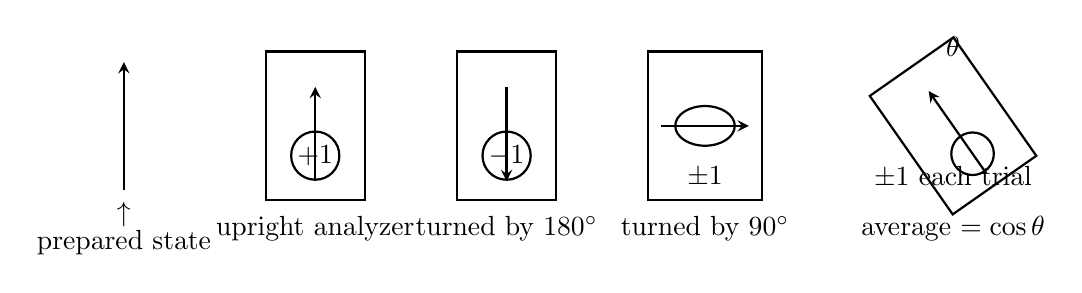
\begin{tikzpicture}[>=stealth,thick,scale=0.90]
\draw[->] (0,0)--(0,1.8);
\node at (0,-0.35) {\(\uparrow\)};
\node at (0,-0.75) {prepared state};

\draw (2.0,-0.15) rectangle (3.4,1.95);
\draw (2.7,0.48) circle (0.34);
\draw[->] (2.7,0.12)--(2.7,1.45);
\node at (2.7,0.48) {\(+1\)};
\node at (2.7,-0.55) {upright analyzer};

\draw (4.7,-0.15) rectangle (6.1,1.95);
\draw (5.4,0.48) circle (0.34);
\draw[->] (5.4,1.45)--(5.4,0.12);
\node at (5.4,0.48) {\(-1\)};
\node at (5.4,-0.55) {turned by \(180^\circ\)};

\draw (7.4,-0.15) rectangle (9.0,1.95);
\draw (8.2,0.90) ellipse (0.42 and 0.28);
\draw[->] (7.58,0.90)--(8.82,0.90);
\node at (8.2,0.18) {\(\pm 1\)};
\node at (8.2,-0.55) {turned by \(90^\circ\)};

\begin{scope}[shift={(11.7,0.90)},rotate=35]
\draw (-0.72,-1.02) rectangle (0.72,1.02);
\draw (0,-0.48) circle (0.30);
\draw[->] (0,-0.82)--(0,0.60);
\end{scope}
\node at (11.7,0.18) {\(\pm 1\) each trial};
\node at (11.7,-0.55) {average \(=\cos\theta\)};
\node at (11.7,2.02) {\(\theta\)};
\end{tikzpicture}
\caption{Cleaned reconstruction of the detector-orientation experiments. The redraw follows the transcript's logic rather than every literal chalk arrow.}
\end{figure}

\subsection{Question \& Answer}

\paragraph{Question.} If the qubit has been prepared ``up,'' why does a sideways detector not read \(0\), the way a classical detector would read the horizontal component of an ordinary upward pointer?

\paragraph{Answer.} Because the qubit is not behaving like an ordinary classical pointer. The sideways measurement still yields only the discrete outcomes \(+1\) and \(-1\). The first sideways result is random. If it happens to be \(+1\), then a repeated sideways measurement confirms that \(+1\) again and again. But if we now rotate the detector back to the original upright orientation, the result becomes random once more. The measurement has prepared the qubit relative to the new axis, not revealed a pre-existing classical component.

This is the main conceptual shock of the lecture. Classical component language works for averages, but it fails at the level of individual experiments. A classical upward pointer has zero horizontal component. A quantum-mechanical ``up'' qubit does not yield \(0\) under a sideways measurement, ever. It yields only \(+1\) or \(-1\).

\section{Ensembles, Rotated Detectors, and the \(\cos\theta\) Law}

At this point the lecture makes a distinction that must not be blurred. There is a difference between confirming a measurement on one already measured qubit and determining statistics across many identically prepared qubits.

For the sideways analyzer, a single run gives either \(+1\) or \(-1\). If we repeat the same sideways measurement on that same qubit, we only confirm the already established result. To see the underlying law, we must prepare many qubits in the same initial state and measure each one once.

For the \(90^\circ\) case, the lecture's statement is:
\begin{equation}
\text{each trial gives }+1\text{ or }-1,
\qquad
\text{but the ensemble average is }0.
\end{equation}
This is not because the apparatus is secretly returning intermediate values. It never does. The average is zero only because, over many identically prepared trials, there are as many \(+1\)'s as \(-1\)'s.

If we now rotate the detector by an arbitrary angle \(\theta\) relative to the preparation axis, the same pattern survives. Each single trial still gives only \(+1\) or \(-1\), but the average now depends smoothly on \(\theta\). As a convenient editorial shorthand, let
\begin{equation}
\overline{\sigma}(\theta)
\end{equation}
denote the ensemble average of the readout for an analyzer tilted by \(\theta\). Then the lecture's empirical rule is
\begin{align}
\overline{\sigma}(0) &= 1,\\
\overline{\sigma}\!\left(\frac{\pi}{2}\right) &= 0,\\
\overline{\sigma}(\pi) &= -1,\\
\overline{\sigma}(\theta) &= \cos\theta.
\end{align}
The lecture does \emph{not} yet derive detailed probabilities for \(+1\) and \(-1\); it gives only the average. That restraint should be preserved here. The point of the experiment is already striking enough: the average behaves as though one were taking the component of a classical vector, but the individual measurements never do.

In fact the lecture emphasizes the two sides together. If the detector is nearly upright, then mostly we see \(+1\), with an occasional \(-1\). If it is nearly upside down, then mostly we see \(-1\), with an occasional \(+1\). At no stage does the detector return a continuum of values. The continuum appears only after averaging.

\subsection{Question \& Answer}

\paragraph{Question.} Why do we need a collection of identically prepared qubits? If nothing happens between measurements, why can we not keep using the same qubit and recover the average from repeated measurements on it?

\paragraph{Answer.} Because repeated measurements with the same detector do not generate a distribution. They only confirm the outcome of the first measurement. Once a tilted analyzer has produced \(+1\) or \(-1\), the qubit has been prepared relative to that tilted axis, and repeating the same tilted measurement merely reproduces the same answer. To learn the statistical law, we need many qubits prepared in the same initial state and measured once each.

The lecture later answers a related question about the sequence of outcomes. For the purposes of this first discussion, the trials are taken to be random and uncorrelated from one prepared qubit to the next. The interesting structure is in the mean, not in higher-order correlations.

This is also where Susskind explicitly postpones the more interpretive language. One can say, if one likes, that the measurement has collapsed the state, but the lecture refuses to lean on that vocabulary yet. Operationally, it is enough to say that the first measurement changes the system, and the second measurement, if carried out immediately in the same orientation, merely keeps what the first one has done.

The same kind of postponement applies to the apparatus itself. Strictly speaking, the detector is also a physical system and ought eventually to be treated quantum mechanically. The lecture acknowledges this point but sets it aside. For now, the world is provisionally divided into detectors and systems. The complication of combining them into a single quantum description is deferred to a later stage.

The lecture now leaves us with the puzzle in its clearest form. The average behavior looks vector-like. The single-shot outcomes do not. That is exactly the moment when the mathematics of vector spaces is brought onto the stage.

\section{From Pointers to Complex Vector Spaces}

Susskind begins the mathematical interlude by separating two meanings of the word \emph{vector}. An ordinary arrow in physical space is something we can picture geometrically. To keep that meaning distinct, he gives it a private name: a \emph{pointer}. The vectors that quantum mechanics needs are more abstract. They are not necessarily arrows in ordinary three-dimensional space at all.

\begin{definition}
A vector space is a collection of mathematical objects with the following basic properties:

\begin{enumerate}
\item vectors can be added, and the sum stays in the same space;
\item vectors can be multiplied by scalars, and the result stays in the same space;
\item there is a zero vector;
\item addition is commutative.
\end{enumerate}
\end{definition}

The lecture stresses closure under addition and scalar multiplication, and then fills in the zero vector and commutativity when asked. Real numbers provide a real vector space: they are closed under addition and multiplication by real numbers. Complex numbers provide a complex vector space: they are closed under addition and multiplication by complex numbers. The lecture also remarks, briefly, that complex-valued functions of a real variable form a vector space as well. That is an important enlargement of the idea, but here it is only a signpost. The main concrete model of the lecture is simpler.

\begin{figure}[ht]
\centering

\includegraphics[width=0.86\textwidth]{lecture_01_figure_05.png}
\caption{Two-component complex column-vector operations.}
\end{figure}

We consider pairs of complex numbers arranged in a column:
\begin{equation}
|\alpha\rangle
\leftrightarrow
\begin{pmatrix}
\alpha_1\\
\alpha_2
\end{pmatrix},
\qquad
\alpha_1,\alpha_2\in\mathbb{C}.
\end{equation}
If
\[
|\beta\rangle
\leftrightarrow
\begin{pmatrix}
\beta_1\\
\beta_2
\end{pmatrix},
\]
then the board gives the rules
\begin{align}
\begin{pmatrix}
\alpha_1\\
\alpha_2
\end{pmatrix}
+
\begin{pmatrix}
\beta_1\\
\beta_2
\end{pmatrix}
&=
\begin{pmatrix}
\alpha_1+\beta_1\\
\alpha_2+\beta_2
\end{pmatrix},\\
z
\begin{pmatrix}
\alpha_1\\
\alpha_2
\end{pmatrix}
&=
\begin{pmatrix}
z\alpha_1\\
z\alpha_2
\end{pmatrix},
\qquad
z\in\mathbb{C}.
\end{align}
This is the concrete realization that the lecture wants us to hold on to. Columns of length two form one vector space. Columns of length three form another. One does not add a two-entry column to a three-entry column, because there is no rule for doing so.

The zero vector is simply
\begin{equation}
|0\rangle=
\begin{pmatrix}
0\\
0
\end{pmatrix},
\qquad
|\alpha\rangle+|0\rangle=|\alpha\rangle,
\end{equation}
and commutativity follows because the entries are ordinary complex numbers:
\begin{equation}
|\alpha\rangle+|\beta\rangle=|\beta\rangle+|\alpha\rangle.
\end{equation}

Now Dirac notation enters more seriously. The abstract vectors are \emph{kets}, written \( |A\rangle \). For each ket there is a corresponding element in the dual vector space, written \( \langle A| \), and called a \emph{bra}. The correspondence preserves addition and conjugates scalars:
\begin{align}
\langle A+B| &= \langle A|+\langle B|,\\
\langle zA| &= z^*\langle A|.
\end{align}
For the concrete two-component column,
\begin{equation}
|\alpha\rangle
\leftrightarrow
\begin{pmatrix}
\alpha_1\\
\alpha_2
\end{pmatrix}
\qquad\Longrightarrow\qquad
\langle \alpha|
\leftrightarrow
\begin{pmatrix}
\alpha_1^* & \alpha_2^*
\end{pmatrix}.
\end{equation}
The row form is only a device for keeping track of which space the object lives in, but it is a very convenient one.

With bras and kets in hand, the lecture defines the inner product. If
\[
\langle\beta|
\leftrightarrow
\begin{pmatrix}
\beta_1^* & \beta_2^*
\end{pmatrix},
\qquad
|\alpha\rangle
\leftrightarrow
\begin{pmatrix}
\alpha_1\\
\alpha_2
\end{pmatrix},
\]
then
\begin{equation}
\langle\beta|\alpha\rangle
=
\beta_1^*\alpha_1+\beta_2^*\alpha_2.
\end{equation}
This is the complex analogue of the dot product for pointers: multiply corresponding components and add, except that the bra contributes complex-conjugated components.

\begin{proposition}
For the two-component complex column model,
\begin{equation}
\langle A|B\rangle=\langle B|A\rangle^*.
\end{equation}
Moreover,
\begin{equation}
\langle \alpha|\alpha\rangle
=
|\alpha_1|^2+|\alpha_2|^2,
\end{equation}
which is real and nonnegative.
\end{proposition}

\begin{proof}
Write
\[
\langle\beta|\alpha\rangle=\beta_1^*\alpha_1+\beta_2^*\alpha_2.
\]
Interchanging \(\alpha\) and \(\beta\) gives
\[
\langle\alpha|\beta\rangle=\alpha_1^*\beta_1+\alpha_2^*\beta_2,
\]
which is the complex conjugate of the previous expression. Hence
\[
\langle\beta|\alpha\rangle=\langle\alpha|\beta\rangle^*.
\]
Now set \(\beta=\alpha\). Then
\[
\langle\alpha|\alpha\rangle
=
\alpha_1^*\alpha_1+\alpha_2^*\alpha_2
=
|\alpha_1|^2+|\alpha_2|^2.
\]
Each term is real and nonnegative, so the whole expression is real and nonnegative.
\end{proof}

The lecture interprets \(\langle A|A\rangle\) as the square of the length of the vector. Thus even though the components are complex, the length is real and positive.

Orthogonality is then defined in the expected way.

\begin{definition}
Two vectors are orthogonal if their inner product vanishes:
\begin{equation}
\langle A|B\rangle=0.
\end{equation}
\end{definition}

\subsection{Question \& Answer}

\paragraph{Question.} Does the order matter? Is \(\langle B|A\rangle\) the same as \(\langle A|B\rangle\)?

\paragraph{Answer.} No. In a complex vector space the two expressions are not generally equal; they are complex conjugates of one another:
\[
\langle A|B\rangle=\langle B|A\rangle^*.
\]
But this is enough to make orthogonality symmetric. If \(\langle A|B\rangle=0\), then \(\langle B|A\rangle=0^*=0\). So orthogonality does not depend on order, even though the inner product itself does.

Finally the lecture turns to dimension. Rather than taking dimension to mean ``number of components'' from the outset, it defines it abstractly as the maximal number of mutually orthogonal nonzero vectors in the space. In the concrete two-component model, a simple orthogonal pair is
\begin{equation}
|e_1\rangle=
\begin{pmatrix}
1\\
0
\end{pmatrix},
\qquad
|e_2\rangle=
\begin{pmatrix}
0\\
1
\end{pmatrix},
\qquad
\langle e_1|e_2\rangle=0.
\end{equation}
Once we have found two mutually orthogonal nonzero vectors in this space, there is no third nonzero vector orthogonal to both. Thus the space is two-dimensional. In this example, the abstract definition agrees with the obvious concrete one: the dimension equals the number of components in the column.

The lecture closes the mathematical interlude by hinting that there is still more structure to come. There will be other products of vectors, including outer products that produce matrices, and the general ideas will later be extended to vector spaces of functions. But the central point of tonight's interlude is already in place: the space of states is a complex vector space, not a set.

\section{Summary}

This first lecture places two blackboards side by side. On one blackboard are the experiments. A qubit yields only the two outcomes \(+1\) and \(-1\). A repeated measurement in the same orientation confirms and therefore prepares a state. Turning the analyzer by \(180^\circ\) flips the sign. Turning it by \(90^\circ\) destroys classical definiteness and gives random \(\pm1\) outcomes with zero mean. Turning it by an arbitrary angle \(\theta\) produces an ensemble average \(\cos\theta\).

On the other blackboard is the mathematics. Classical state spaces are sets, and classical logical operations are set-theoretic operations on subsets. Quantum state spaces are different. They are complex vector spaces, with kets, bras, inner products, norms, orthogonality, and dimension. The lecture does not yet weld these two stories together completely. It prepares them. Next time the abstract vector-space machinery will be brought back to the qubit experiments and made to represent their strange logic directly.